\providecommand{\main}{../../..}
\documentclass[\main/main.tex]{subfiles}
\begin{document}
\subsection{Exercise 2}
Given a finite zero sum game represented in the following matrix:

\begin{table}
  \begin{tabular}{L|LLLL}
    f   & b_1 & b_2 & b_3 & b_4 \\
    \hline
    a_1 & 50  & 10  & 90  & 30  \\
    a_2 & 70  & 120 & 40  & 80
  \end{tabular}
\end{table}

\begin{enumerate}[a)]
  \item Determine the optimal strategy for the row player.
  \item Determine the optimal strategy for the column player.
\end{enumerate}

\subsection{Resolution exercise 2}
\subsubsection*{Identification of dominated strategies}
There are no dominated strategies.

\subsubsection*{Optimal strategies}
\fig{
  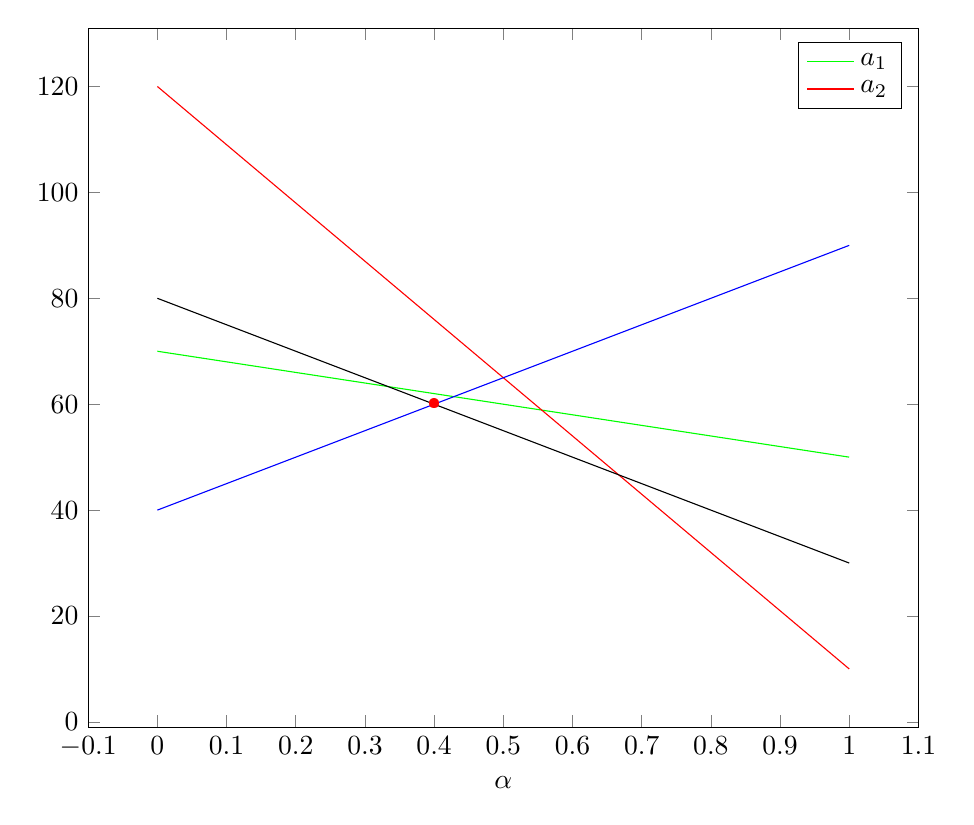
\begin{tikzpicture}
    \begin{axis}[
        width=\textwidth,
        xlabel=$\alpha$,
        samples=100,
        domain=0:1
      ]
      \addplot[mark=none,color=green]{50*x+70*(1-x)};
      \addplot[mark=none,color=red]{10*x+120*(1-x)};
      \addplot[mark=none,color=blue]{90*x+40*(1-x)};
      \addplot[mark=none,color=black]{30*x+80*(1-x)};
      \node[red] at (0.4,60) {\textbullet};
      \legend{$a_1$,$a_2$}
    \end{axis}
  \end{tikzpicture}
  \caption{The optimal strategy for the row player is $(0.3,8)$}
}{}[1]{\caption{Optimal strategies}}

\end{document}